\documentclass{report}

%%%%%%%%%%%%%%%%%%%%%%%%%%%%%%%%%
% PACKAGE IMPORTS
%%%%%%%%%%%%%%%%%%%%%%%%%%%%%%%%%


\usepackage[tmargin=2cm,rmargin=1in,lmargin=1in,margin=0.85in,bmargin=2cm,footskip=.2in]{geometry}
\usepackage{amsmath,amsfonts,amsthm,amssymb,mathtools}
\usepackage[varbb]{newpxmath}
\usepackage{xfrac}
\usepackage[makeroom]{cancel}
\usepackage{mathtools}
\usepackage{bookmark}
\usepackage{enumitem}
\usepackage{hyperref,theoremref}
\hypersetup{
	pdftitle={Assignment},
	colorlinks=true, linkcolor=doc!90,
	bookmarksnumbered=true,
	bookmarksopen=true
}
\usepackage[most,many,breakable]{tcolorbox}
\usepackage{xcolor}
\usepackage{varwidth}
\usepackage{varwidth}
\usepackage{etoolbox}
%\usepackage{authblk}
\usepackage{nameref}
\usepackage{multicol,array}
\usepackage{tikz-cd}
\usepackage[ruled,vlined,linesnumbered]{algorithm2e}
\usepackage{comment} % enables the use of multi-line comments (\ifx \fi) 
\usepackage{import}
\usepackage{xifthen}
\usepackage{pdfpages}
\usepackage{transparent}

\newcommand\mycommfont[1]{\footnotesize\ttfamily\textcolor{blue}{#1}}
\SetCommentSty{mycommfont}
\newcommand{\incfig}[1]{%
    \def\svgwidth{\columnwidth}
    \import{./figures/}{#1.pdf_tex}
}

\usepackage{tikzsymbols}
\renewcommand\qedsymbol{$\Laughey$}


%\usepackage{import}
%\usepackage{xifthen}
%\usepackage{pdfpages}
%\usepackage{transparent}


%%%%%%%%%%%%%%%%%%%%%%%%%%%%%%
% SELF MADE COLORS
%%%%%%%%%%%%%%%%%%%%%%%%%%%%%%



\definecolor{myg}{RGB}{56, 140, 70}
\definecolor{myb}{RGB}{45, 111, 177}
\definecolor{myr}{RGB}{199, 68, 64}
\definecolor{mytheorembg}{HTML}{F2F2F9}
\definecolor{mytheoremfr}{HTML}{00007B}
\definecolor{mylenmabg}{HTML}{FFFAF8}
\definecolor{mylenmafr}{HTML}{983b0f}
\definecolor{mypropbg}{HTML}{f2fbfc}
\definecolor{mypropfr}{HTML}{191971}
\definecolor{myexamplebg}{HTML}{F2FBF8}
\definecolor{myexamplefr}{HTML}{88D6D1}
\definecolor{myexampleti}{HTML}{2A7F7F}
\definecolor{mydefinitbg}{HTML}{E5E5FF}
\definecolor{mydefinitfr}{HTML}{3F3FA3}
\definecolor{notesgreen}{RGB}{0,162,0}
\definecolor{myp}{RGB}{197, 92, 212}
\definecolor{mygr}{HTML}{2C3338}
\definecolor{myred}{RGB}{127,0,0}
\definecolor{myyellow}{RGB}{169,121,69}
\definecolor{myexercisebg}{HTML}{F2FBF8}
\definecolor{myexercisefg}{HTML}{88D6D1}


%%%%%%%%%%%%%%%%%%%%%%%%%%%%
% TCOLORBOX SETUPS
%%%%%%%%%%%%%%%%%%%%%%%%%%%%

\setlength{\parindent}{1cm}
%================================
% THEOREM BOX
%================================

\tcbuselibrary{theorems,skins,hooks}
\newtcbtheorem[number within=section]{Theorem}{Theorem}
{%
	enhanced,
	breakable,
	colback = mytheorembg,
	frame hidden,
	boxrule = 0sp,
	borderline west = {2pt}{0pt}{mytheoremfr},
	sharp corners,
	detach title,
	before upper = \tcbtitle\par\smallskip,
	coltitle = mytheoremfr,
	fonttitle = \bfseries\sffamily,
	description font = \mdseries,
	separator sign none,
	segmentation style={solid, mytheoremfr},
}
{th}

\tcbuselibrary{theorems,skins,hooks}
\newtcbtheorem[number within=chapter]{theorem}{Theorem}
{%
	enhanced,
	breakable,
	colback = mytheorembg,
	frame hidden,
	boxrule = 0sp,
	borderline west = {2pt}{0pt}{mytheoremfr},
	sharp corners,
	detach title,
	before upper = \tcbtitle\par\smallskip,
	coltitle = mytheoremfr,
	fonttitle = \bfseries\sffamily,
	description font = \mdseries,
	separator sign none,
	segmentation style={solid, mytheoremfr},
}
{th}


\tcbuselibrary{theorems,skins,hooks}
\newtcolorbox{Theoremcon}
{%
	enhanced
	,breakable
	,colback = mytheorembg
	,frame hidden
	,boxrule = 0sp
	,borderline west = {2pt}{0pt}{mytheoremfr}
	,sharp corners
	,description font = \mdseries
	,separator sign none
}

%================================
% Corollery
%================================
\tcbuselibrary{theorems,skins,hooks}
\newtcbtheorem[number within=section]{Corollary}{Corollary}
{%
	enhanced
	,breakable
	,colback = myp!10
	,frame hidden
	,boxrule = 0sp
	,borderline west = {2pt}{0pt}{myp!85!black}
	,sharp corners
	,detach title
	,before upper = \tcbtitle\par\smallskip
	,coltitle = myp!85!black
	,fonttitle = \bfseries\sffamily
	,description font = \mdseries
	,separator sign none
	,segmentation style={solid, myp!85!black}
}
{th}
\tcbuselibrary{theorems,skins,hooks}
\newtcbtheorem[number within=chapter]{corollary}{Corollary}
{%
	enhanced
	,breakable
	,colback = myp!10
	,frame hidden
	,boxrule = 0sp
	,borderline west = {2pt}{0pt}{myp!85!black}
	,sharp corners
	,detach title
	,before upper = \tcbtitle\par\smallskip
	,coltitle = myp!85!black
	,fonttitle = \bfseries\sffamily
	,description font = \mdseries
	,separator sign none
	,segmentation style={solid, myp!85!black}
}
{th}


%================================
% LENMA
%================================

\tcbuselibrary{theorems,skins,hooks}
\newtcbtheorem[number within=section]{Lenma}{Lenma}
{%
	enhanced,
	breakable,
	colback = mylenmabg,
	frame hidden,
	boxrule = 0sp,
	borderline west = {2pt}{0pt}{mylenmafr},
	sharp corners,
	detach title,
	before upper = \tcbtitle\par\smallskip,
	coltitle = mylenmafr,
	fonttitle = \bfseries\sffamily,
	description font = \mdseries,
	separator sign none,
	segmentation style={solid, mylenmafr},
}
{th}

\tcbuselibrary{theorems,skins,hooks}
\newtcbtheorem[number within=chapter]{lenma}{Lenma}
{%
	enhanced,
	breakable,
	colback = mylenmabg,
	frame hidden,
	boxrule = 0sp,
	borderline west = {2pt}{0pt}{mylenmafr},
	sharp corners,
	detach title,
	before upper = \tcbtitle\par\smallskip,
	coltitle = mylenmafr,
	fonttitle = \bfseries\sffamily,
	description font = \mdseries,
	separator sign none,
	segmentation style={solid, mylenmafr},
}
{th}


%================================
% PROPOSITION
%================================

\tcbuselibrary{theorems,skins,hooks}
\newtcbtheorem[number within=section]{Prop}{Proposition}
{%
	enhanced,
	breakable,
	colback = mypropbg,
	frame hidden,
	boxrule = 0sp,
	borderline west = {2pt}{0pt}{mypropfr},
	sharp corners,
	detach title,
	before upper = \tcbtitle\par\smallskip,
	coltitle = mypropfr,
	fonttitle = \bfseries\sffamily,
	description font = \mdseries,
	separator sign none,
	segmentation style={solid, mypropfr},
}
{th}

\tcbuselibrary{theorems,skins,hooks}
\newtcbtheorem[number within=chapter]{prop}{Proposition}
{%
	enhanced,
	breakable,
	colback = mypropbg,
	frame hidden,
	boxrule = 0sp,
	borderline west = {2pt}{0pt}{mypropfr},
	sharp corners,
	detach title,
	before upper = \tcbtitle\par\smallskip,
	coltitle = mypropfr,
	fonttitle = \bfseries\sffamily,
	description font = \mdseries,
	separator sign none,
	segmentation style={solid, mypropfr},
}
{th}


%================================
% CLAIM
%================================

\tcbuselibrary{theorems,skins,hooks}
\newtcbtheorem[number within=section]{claim}{Claim}
{%
	enhanced
	,breakable
	,colback = myg!10
	,frame hidden
	,boxrule = 0sp
	,borderline west = {2pt}{0pt}{myg}
	,sharp corners
	,detach title
	,before upper = \tcbtitle\par\smallskip
	,coltitle = myg!85!black
	,fonttitle = \bfseries\sffamily
	,description font = \mdseries
	,separator sign none
	,segmentation style={solid, myg!85!black}
}
{th}



%================================
% Exercise
%================================

\tcbuselibrary{theorems,skins,hooks}
\newtcbtheorem[number within=section]{Exercise}{Exercise}
{%
	enhanced,
	breakable,
	colback = myexercisebg,
	frame hidden,
	boxrule = 0sp,
	borderline west = {2pt}{0pt}{myexercisefg},
	sharp corners,
	detach title,
	before upper = \tcbtitle\par\smallskip,
	coltitle = myexercisefg,
	fonttitle = \bfseries\sffamily,
	description font = \mdseries,
	separator sign none,
	segmentation style={solid, myexercisefg},
}
{th}

\tcbuselibrary{theorems,skins,hooks}
\newtcbtheorem[number within=chapter]{exercise}{Exercise}
{%
	enhanced,
	breakable,
	colback = myexercisebg,
	frame hidden,
	boxrule = 0sp,
	borderline west = {2pt}{0pt}{myexercisefg},
	sharp corners,
	detach title,
	before upper = \tcbtitle\par\smallskip,
	coltitle = myexercisefg,
	fonttitle = \bfseries\sffamily,
	description font = \mdseries,
	separator sign none,
	segmentation style={solid, myexercisefg},
}
{th}

%================================
% EXAMPLE BOX
%================================

\newtcbtheorem[number within=section]{Example}{Example}
{%
	colback = myexamplebg
	,breakable
	,colframe = myexamplefr
	,coltitle = myexampleti
	,boxrule = 1pt
	,sharp corners
	,detach title
	,before upper=\tcbtitle\par\smallskip
	,fonttitle = \bfseries
	,description font = \mdseries
	,separator sign none
	,description delimiters parenthesis
}
{ex}

\newtcbtheorem[number within=chapter]{example}{Example}
{%
	colback = myexamplebg
	,breakable
	,colframe = myexamplefr
	,coltitle = myexampleti
	,boxrule = 1pt
	,sharp corners
	,detach title
	,before upper=\tcbtitle\par\smallskip
	,fonttitle = \bfseries
	,description font = \mdseries
	,separator sign none
	,description delimiters parenthesis
}
{ex}

%================================
% DEFINITION BOX
%================================

\newtcbtheorem[number within=section]{Definition}{Definition}{enhanced,
	before skip=2mm,after skip=2mm, colback=red!5,colframe=red!80!black,boxrule=0.5mm,
	attach boxed title to top left={xshift=1cm,yshift*=1mm-\tcboxedtitleheight}, varwidth boxed title*=-3cm,
	boxed title style={frame code={
					\path[fill=tcbcolback]
					([yshift=-1mm,xshift=-1mm]frame.north west)
					arc[start angle=0,end angle=180,radius=1mm]
					([yshift=-1mm,xshift=1mm]frame.north east)
					arc[start angle=180,end angle=0,radius=1mm];
					\path[left color=tcbcolback!60!black,right color=tcbcolback!60!black,
						middle color=tcbcolback!80!black]
					([xshift=-2mm]frame.north west) -- ([xshift=2mm]frame.north east)
					[rounded corners=1mm]-- ([xshift=1mm,yshift=-1mm]frame.north east)
					-- (frame.south east) -- (frame.south west)
					-- ([xshift=-1mm,yshift=-1mm]frame.north west)
					[sharp corners]-- cycle;
				},interior engine=empty,
		},
	fonttitle=\bfseries,
	title={#2},#1}{def}
\newtcbtheorem[number within=chapter]{definition}{Definition}{enhanced,
	before skip=2mm,after skip=2mm, colback=red!5,colframe=red!80!black,boxrule=0.5mm,
	attach boxed title to top left={xshift=1cm,yshift*=1mm-\tcboxedtitleheight}, varwidth boxed title*=-3cm,
	boxed title style={frame code={
					\path[fill=tcbcolback]
					([yshift=-1mm,xshift=-1mm]frame.north west)
					arc[start angle=0,end angle=180,radius=1mm]
					([yshift=-1mm,xshift=1mm]frame.north east)
					arc[start angle=180,end angle=0,radius=1mm];
					\path[left color=tcbcolback!60!black,right color=tcbcolback!60!black,
						middle color=tcbcolback!80!black]
					([xshift=-2mm]frame.north west) -- ([xshift=2mm]frame.north east)
					[rounded corners=1mm]-- ([xshift=1mm,yshift=-1mm]frame.north east)
					-- (frame.south east) -- (frame.south west)
					-- ([xshift=-1mm,yshift=-1mm]frame.north west)
					[sharp corners]-- cycle;
				},interior engine=empty,
		},
	fonttitle=\bfseries,
	title={#2},#1}{def}



%================================
% Solution BOX
%================================

\makeatletter
\newtcbtheorem{question}{Question}{enhanced,
	breakable,
	colback=white,
	colframe=myb!80!black,
	attach boxed title to top left={yshift*=-\tcboxedtitleheight},
	fonttitle=\bfseries,
	title={#2},
	boxed title size=title,
	boxed title style={%
			sharp corners,
			rounded corners=northwest,
			colback=tcbcolframe,
			boxrule=0pt,
		},
	underlay boxed title={%
			\path[fill=tcbcolframe] (title.south west)--(title.south east)
			to[out=0, in=180] ([xshift=5mm]title.east)--
			(title.center-|frame.east)
			[rounded corners=\kvtcb@arc] |-
			(frame.north) -| cycle;
		},
	#1
}{def}
\makeatother

%================================
% SOLUTION BOX
%================================

\makeatletter
\newtcolorbox{solution}{enhanced,
	breakable,
	colback=white,
	colframe=myg!80!black,
	attach boxed title to top left={yshift*=-\tcboxedtitleheight},
	title=Solution,
	boxed title size=title,
	boxed title style={%
			sharp corners,
			rounded corners=northwest,
			colback=tcbcolframe,
			boxrule=0pt,
		},
	underlay boxed title={%
			\path[fill=tcbcolframe] (title.south west)--(title.south east)
			to[out=0, in=180] ([xshift=5mm]title.east)--
			(title.center-|frame.east)
			[rounded corners=\kvtcb@arc] |-
			(frame.north) -| cycle;
		},
}
\makeatother

%================================
% Question BOX
%================================

\makeatletter
\newtcbtheorem{qstion}{Question}{enhanced,
	breakable,
	colback=white,
	colframe=mygr,
	attach boxed title to top left={yshift*=-\tcboxedtitleheight},
	fonttitle=\bfseries,
	title={#2},
	boxed title size=title,
	boxed title style={%
			sharp corners,
			rounded corners=northwest,
			colback=tcbcolframe,
			boxrule=0pt,
		},
	underlay boxed title={%
			\path[fill=tcbcolframe] (title.south west)--(title.south east)
			to[out=0, in=180] ([xshift=5mm]title.east)--
			(title.center-|frame.east)
			[rounded corners=\kvtcb@arc] |-
			(frame.north) -| cycle;
		},
	#1
}{def}
\makeatother

\newtcbtheorem[number within=chapter]{wconc}{Wrong Concept}{
	breakable,
	enhanced,
	colback=white,
	colframe=myr,
	arc=0pt,
	outer arc=0pt,
	fonttitle=\bfseries\sffamily\large,
	colbacktitle=myr,
	attach boxed title to top left={},
	boxed title style={
			enhanced,
			skin=enhancedfirst jigsaw,
			arc=3pt,
			bottom=0pt,
			interior style={fill=myr}
		},
	#1
}{def}



%================================
% NOTE BOX
%================================

\usetikzlibrary{arrows,calc,shadows.blur}
\tcbuselibrary{skins}
\newtcolorbox{note}[1][]{%
	enhanced jigsaw,
	colback=gray!20!white,%
	colframe=gray!80!black,
	size=small,
	boxrule=1pt,
	title=\textbf{Note:},
	halign title=flush center,
	coltitle=black,
	breakable,
	drop shadow=black!50!white,
	attach boxed title to top left={xshift=1cm,yshift=-\tcboxedtitleheight/2,yshifttext=-\tcboxedtitleheight/2},
	minipage boxed title=1.5cm,
	boxed title style={%
			colback=white,
			size=fbox,
			boxrule=1pt,
			boxsep=2pt,
			underlay={%
					\coordinate (dotA) at ($(interior.west) + (-0.5pt,0)$);
					\coordinate (dotB) at ($(interior.east) + (0.5pt,0)$);
					\begin{scope}
						\clip (interior.north west) rectangle ([xshift=3ex]interior.east);
						\filldraw [white, blur shadow={shadow opacity=60, shadow yshift=-.75ex}, rounded corners=2pt] (interior.north west) rectangle (interior.south east);
					\end{scope}
					\begin{scope}[gray!80!black]
						\fill (dotA) circle (2pt);
						\fill (dotB) circle (2pt);
					\end{scope}
				},
		},
	#1,
}

%%%%%%%%%%%%%%%%%%%%%%%%%%%%%%
% SELF MADE COMMANDS
%%%%%%%%%%%%%%%%%%%%%%%%%%%%%%


\newcommand{\thm}[2]{\begin{Theorem}{#1}{}#2\end{Theorem}}
\newcommand{\cor}[2]{\begin{Corollary}{#1}{}#2\end{Corollary}}
\newcommand{\mlenma}[2]{\begin{Lenma}{#1}{}#2\end{Lenma}}
\newcommand{\mprop}[2]{\begin{Prop}{#1}{}#2\end{Prop}}
\newcommand{\clm}[3]{\begin{claim}{#1}{#2}#3\end{claim}}
\newcommand{\wc}[2]{\begin{wconc}{#1}{}\setlength{\parindent}{1cm}#2\end{wconc}}
\newcommand{\thmcon}[1]{\begin{Theoremcon}{#1}\end{Theoremcon}}
\newcommand{\ex}[2]{\begin{Example}{#1}{}#2\end{Example}}
\newcommand{\dfn}[2]{\begin{Definition}[colbacktitle=red!75!black]{#1}{}#2\end{Definition}}
\newcommand{\dfnc}[2]{\begin{definition}[colbacktitle=red!75!black]{#1}{}#2\end{definition}}
\newcommand{\qs}[2]{\begin{question}{#1}{}#2\end{question}}
\newcommand{\pf}[2]{\begin{myproof}[#1]#2\end{myproof}}
\newcommand{\nt}[1]{\begin{note}#1\end{note}}

\newcommand*\circled[1]{\tikz[baseline=(char.base)]{
		\node[shape=circle,draw,inner sep=1pt] (char) {#1};}}
\newcommand\getcurrentref[1]{%
	\ifnumequal{\value{#1}}{0}
	{??}
	{\the\value{#1}}%
}
\newcommand{\getCurrentSectionNumber}{\getcurrentref{section}}
\newenvironment{myproof}[1][\proofname]{%
	\proof[\bfseries #1: ]%
}{\endproof}

\newcommand{\mclm}[2]{\begin{myclaim}[#1]#2\end{myclaim}}
\newenvironment{myclaim}[1][\claimname]{\proof[\bfseries #1: ]}{}

\newcounter{mylabelcounter}

\makeatletter
\newcommand{\setword}[2]{%
	\phantomsection
	#1\def\@currentlabel{\unexpanded{#1}}\label{#2}%
}
\makeatother




\tikzset{
	symbol/.style={
			draw=none,
			every to/.append style={
					edge node={node [sloped, allow upside down, auto=false]{$#1$}}}
		}
}


% deliminators
\DeclarePairedDelimiter{\abs}{\lvert}{\rvert}
\DeclarePairedDelimiter{\norm}{\lVert}{\rVert}

\DeclarePairedDelimiter{\ceil}{\lceil}{\rceil}
\DeclarePairedDelimiter{\floor}{\lfloor}{\rfloor}
\DeclarePairedDelimiter{\round}{\lfloor}{\rceil}

\newsavebox\diffdbox
\newcommand{\slantedromand}{{\mathpalette\makesl{d}}}
\newcommand{\makesl}[2]{%
\begingroup
\sbox{\diffdbox}{$\mathsurround=0pt#1\mathrm{#2}$}%
\pdfsave
\pdfsetmatrix{1 0 0.2 1}%
\rlap{\usebox{\diffdbox}}%
\pdfrestore
\hskip\wd\diffdbox
\endgroup
}
\newcommand{\dd}[1][]{\ensuremath{\mathop{}\!\ifstrempty{#1}{%
\slantedromand\@ifnextchar^{\hspace{0.2ex}}{\hspace{0.1ex}}}%
{\slantedromand\hspace{0.2ex}^{#1}}}}
\ProvideDocumentCommand\dv{o m g}{%
  \ensuremath{%
    \IfValueTF{#3}{%
      \IfNoValueTF{#1}{%
        \frac{\dd #2}{\dd #3}%
      }{%
        \frac{\dd^{#1} #2}{\dd #3^{#1}}%
      }%
    }{%
      \IfNoValueTF{#1}{%
        \frac{\dd}{\dd #2}%
      }{%
        \frac{\dd^{#1}}{\dd #2^{#1}}%
      }%
    }%
  }%
}
\providecommand*{\pdv}[3][]{\frac{\partial^{#1}#2}{\partial#3^{#1}}}
%  - others
\DeclareMathOperator{\Lap}{\mathcal{L}}
\DeclareMathOperator{\Var}{Var} % varience
\DeclareMathOperator{\Cov}{Cov} % covarience
\DeclareMathOperator{\E}{E} % expected

% Since the amsthm package isn't loaded

% I prefer the slanted \leq
\let\oldleq\leq % save them in case they're every wanted
\let\oldgeq\geq
\renewcommand{\leq}{\leqslant}
\renewcommand{\geq}{\geqslant}

% % redefine matrix env to allow for alignment, use r as default
% \renewcommand*\env@matrix[1][r]{\hskip -\arraycolsep
%     \let\@ifnextchar\new@ifnextchar
%     \array{*\c@MaxMatrixCols #1}}


%\usepackage{framed}
%\usepackage{titletoc}
%\usepackage{etoolbox}
%\usepackage{lmodern}


%\patchcmd{\tableofcontents}{\contentsname}{\sffamily\contentsname}{}{}

%\renewenvironment{leftbar}
%{\def\FrameCommand{\hspace{6em}%
%		{\color{myyellow}\vrule width 2pt depth 6pt}\hspace{1em}}%
%	\MakeFramed{\parshape 1 0cm \dimexpr\textwidth-6em\relax\FrameRestore}\vskip2pt%
%}
%{\endMakeFramed}

%\titlecontents{chapter}
%[0em]{\vspace*{2\baselineskip}}
%{\parbox{4.5em}{%
%		\hfill\Huge\sffamily\bfseries\color{myred}\thecontentspage}%
%	\vspace*{-2.3\baselineskip}\leftbar\textsc{\small\chaptername~\thecontentslabel}\\\sffamily}
%{}{\endleftbar}
%\titlecontents{section}
%[8.4em]
%{\sffamily\contentslabel{3em}}{}{}
%{\hspace{0.5em}\nobreak\itshape\color{myred}\contentspage}
%\titlecontents{subsection}
%[8.4em]
%{\sffamily\contentslabel{3em}}{}{}  
%{\hspace{0.5em}\nobreak\itshape\color{myred}\contentspage}



%%%%%%%%%%%%%%%%%%%%%%%%%%%%%%%%%%%%%%%%%%%
% TABLE OF CONTENTS
%%%%%%%%%%%%%%%%%%%%%%%%%%%%%%%%%%%%%%%%%%%

\usepackage{tikz}
\definecolor{doc}{RGB}{0,60,110}
\usepackage{titletoc}
\contentsmargin{0cm}
\titlecontents{chapter}[3.7pc]
{\addvspace{30pt}%
	\begin{tikzpicture}[remember picture, overlay]%
		\draw[fill=doc!60,draw=doc!60] (-7,-.1) rectangle (-0.9,.5);%
		\pgftext[left,x=-3.5cm,y=0.2cm]{\color{white}\Large\sc\bfseries Chapter\ \thecontentslabel};%
	\end{tikzpicture}\color{doc!60}\large\sc\bfseries}%
{}
{}
{\;\titlerule\;\large\sc\bfseries Page \thecontentspage
	\begin{tikzpicture}[remember picture, overlay]
		\draw[fill=doc!60,draw=doc!60] (2pt,0) rectangle (4,0.1pt);
	\end{tikzpicture}}%
\titlecontents{section}[3.7pc]
{\addvspace{2pt}}
{\contentslabel[\thecontentslabel]{2pc}}
{}
{\hfill\small \thecontentspage}
[]
\titlecontents*{subsection}[3.7pc]
{\addvspace{-1pt}\small}
{}
{}
{\ --- \small\thecontentspage}
[ \textbullet\ ][]

\makeatletter
\renewcommand{\tableofcontents}{%
	\chapter*{%
	  \vspace*{-20\p@}%
	  \begin{tikzpicture}[remember picture, overlay]%
		  \pgftext[right,x=15cm,y=0.2cm]{\color{doc!60}\Huge\sc\bfseries \contentsname};%
		  \draw[fill=doc!60,draw=doc!60] (13,-.75) rectangle (20,1);%
		  \clip (13,-.75) rectangle (20,1);
		  \pgftext[right,x=15cm,y=0.2cm]{\color{white}\Huge\sc\bfseries \contentsname};%
	  \end{tikzpicture}}%
	\@starttoc{toc}}
\makeatother


% My commands %
\newcommand{\innerproduct}[2]{\langle #1, #2 \rangle}
\newcommand{\generators}[1]{\langle #1 \rangle}

%From M275 "Topology" at SJSU
\newcommand{\id}{\mathrm{id}}
\newcommand{\taking}[1]{\xrightarrow{#1}}
\newcommand{\inv}{^{-1}}

%From M170 "Introduction to Graph Theory" at SJSU
\DeclareMathOperator{\diam}{diam}
\DeclareMathOperator{\ord}{ord}
\newcommand{\defeq}{\overset{\mathrm{def}}{=}}

%From the USAMO .tex files
\newcommand{\ts}{\textsuperscript}
\newcommand{\dg}{^\circ}
\newcommand{\ii}{\item}

% % From Math 55 and Math 145 at Harvard
% \newenvironment{subproof}[1][Proof]{%
% \begin{proof}[#1] \renewcommand{\qedsymbol}{$\blacksquare$}}%
% {\end{proof}}

\newcommand{\liff}{\leftrightarrow}
\newcommand{\lthen}{\rightarrow}
\newcommand{\opname}{\operatorname}
\newcommand{\surjto}{\twoheadrightarrow}
\newcommand{\injto}{\hookrightarrow}
\newcommand{\On}{\mathrm{On}} % ordinals
\DeclareMathOperator{\img}{im} % Image
\DeclareMathOperator{\Img}{Im} % Image
\DeclareMathOperator{\coker}{coker} % Cokernel
\DeclareMathOperator{\Coker}{Coker} % Cokernel
\DeclareMathOperator{\Ker}{Ker} % Kernel
\DeclareMathOperator{\rank}{rank}
\DeclareMathOperator{\Spec}{Spec} % spectrum
\DeclareMathOperator{\Tr}{Tr} % trace
\DeclareMathOperator{\pr}{pr} % projection
\DeclareMathOperator{\ext}{ext} % extension
\DeclareMathOperator{\pred}{pred} % predecessor
\DeclareMathOperator{\dom}{dom} % domain
\DeclareMathOperator{\ran}{ran} % range
\DeclareMathOperator{\Hom}{Hom} % homomorphism
\DeclareMathOperator{\Mor}{Mor} % morphisms
\DeclareMathOperator{\End}{End} % endomorphism

\newcommand{\eps}{\epsilon}
\newcommand{\veps}{\varepsilon}
\newcommand{\ol}{\overline}
\newcommand{\ul}{\underline}
\newcommand{\wt}{\widetilde}
\newcommand{\wh}{\widehat}
\newcommand{\vocab}[1]{\textbf{\color{blue} #1}}
\providecommand{\half}{\frac{1}{2}}
\newcommand{\dang}{\measuredangle} %% Directed angle
\newcommand{\ray}[1]{\overrightarrow{#1}}
\newcommand{\seg}[1]{\overline{#1}}
\newcommand{\arc}[1]{\wideparen{#1}}
\DeclareMathOperator{\cis}{cis}
\DeclareMathOperator*{\lcm}{lcm}
\DeclareMathOperator*{\argmin}{arg min}
\DeclareMathOperator*{\argmax}{arg max}
\newcommand{\cycsum}{\sum_{\mathrm{cyc}}}
\newcommand{\symsum}{\sum_{\mathrm{sym}}}
\newcommand{\cycprod}{\prod_{\mathrm{cyc}}}
\newcommand{\symprod}{\prod_{\mathrm{sym}}}
\newcommand{\Qed}{\begin{flushright}\qed\end{flushright}}
\newcommand{\parinn}{\setlength{\parindent}{1cm}}
\newcommand{\parinf}{\setlength{\parindent}{0cm}}
% \newcommand{\norm}{\|\cdot\|}
\newcommand{\inorm}{\norm_{\infty}}
\newcommand{\opensets}{\{V_{\alpha}\}_{\alpha\in I}}
\newcommand{\oset}{V_{\alpha}}
\newcommand{\opset}[1]{V_{\alpha_{#1}}}
\newcommand{\lub}{\text{lub}}
\newcommand{\del}[2]{\frac{\partial #1}{\partial #2}}
\newcommand{\Del}[3]{\frac{\partial^{#1} #2}{\partial^{#1} #3}}
\newcommand{\deld}[2]{\dfrac{\partial #1}{\partial #2}}
\newcommand{\Deld}[3]{\dfrac{\partial^{#1} #2}{\partial^{#1} #3}}
\newcommand{\lm}{\lambda}
\newcommand{\uin}{\mathbin{\rotatebox[origin=c]{90}{$\in$}}}
\newcommand{\usubset}{\mathbin{\rotatebox[origin=c]{90}{$\subset$}}}
\newcommand{\lt}{\left}
\newcommand{\rt}{\right}
\newcommand{\bs}[1]{\boldsymbol{#1}}
\newcommand{\exs}{\exists}
\newcommand{\st}{\strut}
\newcommand{\dps}[1]{\displaystyle{#1}}

\newcommand{\sol}{\setlength{\parindent}{0cm}\textbf{\textit{Solution:}}\setlength{\parindent}{1cm} }
\newcommand{\solve}[1]{\setlength{\parindent}{0cm}\textbf{\textit{Solution: }}\setlength{\parindent}{1cm}#1 \Qed}

% Things Lie
\newcommand{\kb}{\mathfrak b}
\newcommand{\kg}{\mathfrak g}
\newcommand{\kh}{\mathfrak h}
\newcommand{\kn}{\mathfrak n}
\newcommand{\ku}{\mathfrak u}
\newcommand{\kz}{\mathfrak z}
\DeclareMathOperator{\Ext}{Ext} % Ext functor
\DeclareMathOperator{\Tor}{Tor} % Tor functor
\newcommand{\gl}{\opname{\mathfrak{gl}}} % frak gl group
\renewcommand{\sl}{\opname{\mathfrak{sl}}} % frak sl group chktex 6

% More script letters etc.
\newcommand{\SA}{\mathcal A}
\newcommand{\SB}{\mathcal B}
\newcommand{\SC}{\mathcal C}
\newcommand{\SF}{\mathcal F}
\newcommand{\SG}{\mathcal G}
\newcommand{\SH}{\mathcal H}
\newcommand{\OO}{\mathcal O}

\newcommand{\SCA}{\mathscr A}
\newcommand{\SCB}{\mathscr B}
\newcommand{\SCC}{\mathscr C}
\newcommand{\SCD}{\mathscr D}
\newcommand{\SCE}{\mathscr E}
\newcommand{\SCF}{\mathscr F}
\newcommand{\SCG}{\mathscr G}
\newcommand{\SCH}{\mathscr H}

% Mathfrak primes
\newcommand{\km}{\mathfrak m}
\newcommand{\kp}{\mathfrak p}
\newcommand{\kq}{\mathfrak q}

% number sets
\newcommand{\RR}[1][]{\ensuremath{\ifstrempty{#1}{\mathbb{R}}{\mathbb{R}^{#1}}}}
\newcommand{\NN}[1][]{\ensuremath{\ifstrempty{#1}{\mathbb{N}}{\mathbb{N}^{#1}}}}
\newcommand{\ZZ}[1][]{\ensuremath{\ifstrempty{#1}{\mathbb{Z}}{\mathbb{Z}^{#1}}}}
\newcommand{\QQ}[1][]{\ensuremath{\ifstrempty{#1}{\mathbb{Q}}{\mathbb{Q}^{#1}}}}
\newcommand{\CC}[1][]{\ensuremath{\ifstrempty{#1}{\mathbb{C}}{\mathbb{C}^{#1}}}}
\newcommand{\PP}[1][]{\ensuremath{\ifstrempty{#1}{\mathbb{P}}{\mathbb{P}^{#1}}}}
\newcommand{\HH}[1][]{\ensuremath{\ifstrempty{#1}{\mathbb{H}}{\mathbb{H}^{#1}}}}
\newcommand{\FF}[1][]{\ensuremath{\ifstrempty{#1}{\mathbb{F}}{\mathbb{F}^{#1}}}}
% expected value
\newcommand{\EE}{\ensuremath{\mathbb{E}}}
\newcommand{\charin}{\text{ char }}
\DeclareMathOperator{\sign}{sign}
\DeclareMathOperator{\Aut}{Aut}
\DeclareMathOperator{\Inn}{Inn}
\DeclareMathOperator{\Syl}{Syl}
\DeclareMathOperator{\Gal}{Gal}
\DeclareMathOperator{\GL}{GL} % General linear group
\DeclareMathOperator{\SL}{SL} % Special linear group

%---------------------------------------
% BlackBoard Math Fonts :-
%---------------------------------------

%Captital Letters
\newcommand{\bbA}{\mathbb{A}}	\newcommand{\bbB}{\mathbb{B}}
\newcommand{\bbC}{\mathbb{C}}	\newcommand{\bbD}{\mathbb{D}}
\newcommand{\bbE}{\mathbb{E}}	\newcommand{\bbF}{\mathbb{F}}
\newcommand{\bbG}{\mathbb{G}}	\newcommand{\bbH}{\mathbb{H}}
\newcommand{\bbI}{\mathbb{I}}	\newcommand{\bbJ}{\mathbb{J}}
\newcommand{\bbK}{\mathbb{K}}	\newcommand{\bbL}{\mathbb{L}}
\newcommand{\bbM}{\mathbb{M}}	\newcommand{\bbN}{\mathbb{N}}
\newcommand{\bbO}{\mathbb{O}}	\newcommand{\bbP}{\mathbb{P}}
\newcommand{\bbQ}{\mathbb{Q}}	\newcommand{\bbR}{\mathbb{R}}
\newcommand{\bbS}{\mathbb{S}}	\newcommand{\bbT}{\mathbb{T}}
\newcommand{\bbU}{\mathbb{U}}	\newcommand{\bbV}{\mathbb{V}}
\newcommand{\bbW}{\mathbb{W}}	\newcommand{\bbX}{\mathbb{X}}
\newcommand{\bbY}{\mathbb{Y}}	\newcommand{\bbZ}{\mathbb{Z}}

%---------------------------------------
% MathCal Fonts :-
%---------------------------------------

%Captital Letters
\newcommand{\mcA}{\mathcal{A}}	\newcommand{\mcB}{\mathcal{B}}
\newcommand{\mcC}{\mathcal{C}}	\newcommand{\mcD}{\mathcal{D}}
\newcommand{\mcE}{\mathcal{E}}	\newcommand{\mcF}{\mathcal{F}}
\newcommand{\mcG}{\mathcal{G}}	\newcommand{\mcH}{\mathcal{H}}
\newcommand{\mcI}{\mathcal{I}}	\newcommand{\mcJ}{\mathcal{J}}
\newcommand{\mcK}{\mathcal{K}}	\newcommand{\mcL}{\mathcal{L}}
\newcommand{\mcM}{\mathcal{M}}	\newcommand{\mcN}{\mathcal{N}}
\newcommand{\mcO}{\mathcal{O}}	\newcommand{\mcP}{\mathcal{P}}
\newcommand{\mcQ}{\mathcal{Q}}	\newcommand{\mcR}{\mathcal{R}}
\newcommand{\mcS}{\mathcal{S}}	\newcommand{\mcT}{\mathcal{T}}
\newcommand{\mcU}{\mathcal{U}}	\newcommand{\mcV}{\mathcal{V}}
\newcommand{\mcW}{\mathcal{W}}	\newcommand{\mcX}{\mathcal{X}}
\newcommand{\mcY}{\mathcal{Y}}	\newcommand{\mcZ}{\mathcal{Z}}


%---------------------------------------
% Bold Math Fonts :-
%---------------------------------------

%Captital Letters
\newcommand{\bmA}{\boldsymbol{A}}	\newcommand{\bmB}{\boldsymbol{B}}
\newcommand{\bmC}{\boldsymbol{C}}	\newcommand{\bmD}{\boldsymbol{D}}
\newcommand{\bmE}{\boldsymbol{E}}	\newcommand{\bmF}{\boldsymbol{F}}
\newcommand{\bmG}{\boldsymbol{G}}	\newcommand{\bmH}{\boldsymbol{H}}
\newcommand{\bmI}{\boldsymbol{I}}	\newcommand{\bmJ}{\boldsymbol{J}}
\newcommand{\bmK}{\boldsymbol{K}}	\newcommand{\bmL}{\boldsymbol{L}}
\newcommand{\bmM}{\boldsymbol{M}}	\newcommand{\bmN}{\boldsymbol{N}}
\newcommand{\bmO}{\boldsymbol{O}}	\newcommand{\bmP}{\boldsymbol{P}}
\newcommand{\bmQ}{\boldsymbol{Q}}	\newcommand{\bmR}{\boldsymbol{R}}
\newcommand{\bmS}{\boldsymbol{S}}	\newcommand{\bmT}{\boldsymbol{T}}
\newcommand{\bmU}{\boldsymbol{U}}	\newcommand{\bmV}{\boldsymbol{V}}
\newcommand{\bmW}{\boldsymbol{W}}	\newcommand{\bmX}{\boldsymbol{X}}
\newcommand{\bmY}{\boldsymbol{Y}}	\newcommand{\bmZ}{\boldsymbol{Z}}
%Small Letters
\newcommand{\bma}{\boldsymbol{a}}	\newcommand{\bmb}{\boldsymbol{b}}
\newcommand{\bmc}{\boldsymbol{c}}	\newcommand{\bmd}{\boldsymbol{d}}
\newcommand{\bme}{\boldsymbol{e}}	\newcommand{\bmf}{\boldsymbol{f}}
\newcommand{\bmg}{\boldsymbol{g}}	\newcommand{\bmh}{\boldsymbol{h}}
\newcommand{\bmi}{\boldsymbol{i}}	\newcommand{\bmj}{\boldsymbol{j}}
\newcommand{\bmk}{\boldsymbol{k}}	\newcommand{\bml}{\boldsymbol{l}}
\newcommand{\bmm}{\boldsymbol{m}}	\newcommand{\bmn}{\boldsymbol{n}}
\newcommand{\bmo}{\boldsymbol{o}}	\newcommand{\bmp}{\boldsymbol{p}}
\newcommand{\bmq}{\boldsymbol{q}}	\newcommand{\bmr}{\boldsymbol{r}}
\newcommand{\bms}{\boldsymbol{s}}	\newcommand{\bmt}{\boldsymbol{t}}
\newcommand{\bmu}{\boldsymbol{u}}	\newcommand{\bmv}{\boldsymbol{v}}
\newcommand{\bmw}{\boldsymbol{w}}	\newcommand{\bmx}{\boldsymbol{x}}
\newcommand{\bmy}{\boldsymbol{y}}	\newcommand{\bmz}{\boldsymbol{z}}

%---------------------------------------
% Scr Math Fonts :-
%---------------------------------------

\newcommand{\sA}{{\mathscr{A}}}   \newcommand{\sB}{{\mathscr{B}}}
\newcommand{\sC}{{\mathscr{C}}}   \newcommand{\sD}{{\mathscr{D}}}
\newcommand{\sE}{{\mathscr{E}}}   \newcommand{\sF}{{\mathscr{F}}}
\newcommand{\sG}{{\mathscr{G}}}   \newcommand{\sH}{{\mathscr{H}}}
\newcommand{\sI}{{\mathscr{I}}}   \newcommand{\sJ}{{\mathscr{J}}}
\newcommand{\sK}{{\mathscr{K}}}   \newcommand{\sL}{{\mathscr{L}}}
\newcommand{\sM}{{\mathscr{M}}}   \newcommand{\sN}{{\mathscr{N}}}
\newcommand{\sO}{{\mathscr{O}}}   \newcommand{\sP}{{\mathscr{P}}}
\newcommand{\sQ}{{\mathscr{Q}}}   \newcommand{\sR}{{\mathscr{R}}}
\newcommand{\sS}{{\mathscr{S}}}   \newcommand{\sT}{{\mathscr{T}}}
\newcommand{\sU}{{\mathscr{U}}}   \newcommand{\sV}{{\mathscr{V}}}
\newcommand{\sW}{{\mathscr{W}}}   \newcommand{\sX}{{\mathscr{X}}}
\newcommand{\sY}{{\mathscr{Y}}}   \newcommand{\sZ}{{\mathscr{Z}}}


%---------------------------------------
% Math Fraktur Font
%---------------------------------------

%Captital Letters
\newcommand{\mfA}{\mathfrak{A}}	\newcommand{\mfB}{\mathfrak{B}}
\newcommand{\mfC}{\mathfrak{C}}	\newcommand{\mfD}{\mathfrak{D}}
\newcommand{\mfE}{\mathfrak{E}}	\newcommand{\mfF}{\mathfrak{F}}
\newcommand{\mfG}{\mathfrak{G}}	\newcommand{\mfH}{\mathfrak{H}}
\newcommand{\mfI}{\mathfrak{I}}	\newcommand{\mfJ}{\mathfrak{J}}
\newcommand{\mfK}{\mathfrak{K}}	\newcommand{\mfL}{\mathfrak{L}}
\newcommand{\mfM}{\mathfrak{M}}	\newcommand{\mfN}{\mathfrak{N}}
\newcommand{\mfO}{\mathfrak{O}}	\newcommand{\mfP}{\mathfrak{P}}
\newcommand{\mfQ}{\mathfrak{Q}}	\newcommand{\mfR}{\mathfrak{R}}
\newcommand{\mfS}{\mathfrak{S}}	\newcommand{\mfT}{\mathfrak{T}}
\newcommand{\mfU}{\mathfrak{U}}	\newcommand{\mfV}{\mathfrak{V}}
\newcommand{\mfW}{\mathfrak{W}}	\newcommand{\mfX}{\mathfrak{X}}
\newcommand{\mfY}{\mathfrak{Y}}	\newcommand{\mfZ}{\mathfrak{Z}}
%Small Letters
\newcommand{\mfa}{\mathfrak{a}}	\newcommand{\mfb}{\mathfrak{b}}
\newcommand{\mfc}{\mathfrak{c}}	\newcommand{\mfd}{\mathfrak{d}}
\newcommand{\mfe}{\mathfrak{e}}	\newcommand{\mff}{\mathfrak{f}}
\newcommand{\mfg}{\mathfrak{g}}	\newcommand{\mfh}{\mathfrak{h}}
\newcommand{\mfi}{\mathfrak{i}}	\newcommand{\mfj}{\mathfrak{j}}
\newcommand{\mfk}{\mathfrak{k}}	\newcommand{\mfl}{\mathfrak{l}}
\newcommand{\mfm}{\mathfrak{m}}	\newcommand{\mfn}{\mathfrak{n}}
\newcommand{\mfo}{\mathfrak{o}}	\newcommand{\mfp}{\mathfrak{p}}
\newcommand{\mfq}{\mathfrak{q}}	\newcommand{\mfr}{\mathfrak{r}}
\newcommand{\mfs}{\mathfrak{s}}	\newcommand{\mft}{\mathfrak{t}}
\newcommand{\mfu}{\mathfrak{u}}	\newcommand{\mfv}{\mathfrak{v}}
\newcommand{\mfw}{\mathfrak{w}}	\newcommand{\mfx}{\mathfrak{x}}
\newcommand{\mfy}{\mathfrak{y}}	\newcommand{\mfz}{\mathfrak{z}}

\usepackage{xcolor}
\usepackage{tikz-qtree}
\usepackage{graphicx}
\usepackage{cancel}

% Tikz libraries %
\usetikzlibrary{automata, positioning, arrows, shapes.geometric, decorations.pathmorphing}

% Impostazioni Tikz %
\tikzset{
    ->, % makes the edges directed
    >=stealth, % makes the arrow heads bold
    node distance=3cm, % specifies the minimum distance between two nodes. Change if necessary.
    every state/.style={thick, fill=gray!10}, % sets the properties for each ’state’ node
    initial text=$start$, % sets the text that appears on the start arrow
}

%frccina ondulata
\tikzset{
    wavearrow/.style={
        -{Stealth[scale=1.2]}, 
        decorate,
        decoration={snake, amplitude=1mm, segment length=5mm},
        thick
    }
}

% Tikz shapes (manca initial, state e accept) %
\tikzstyle{startstop} = [rectangle, rounded corners, minimum width=3cm, minimum height=1cm,text centered, draw=black, fill=red!30]
\tikzstyle{process} = [rectangle, minimum width=3cm, minimum height=1cm, text centered, draw=black, fill=orange!30]
\tikzstyle{decision} = [diamond, minimum width=3cm, minimum height=1cm, text centered, draw=black, fill=green!30]
\tikzstyle{arrow} = [thick,->,>=stealth]

\tikzstyle{block} = [rectangle, rounded corners, draw, align=center, text width=3cm, minimum height=1cm]
\tikzstyle{arrow} = [thick, ->, >=stealth]
\tikzstyle{stack} = [rectangle, draw, align=center, minimum width=1.3cm, minimum height=0.5cm]


\title{\Huge{Linguaggi di programmazione}\\Appunti}
\author{\huge{Giovanni Palma e Alex Basta}}
\date{}
\pagenumbering{gobble}

\graphicspath{{paginette2/img/}}

\begin{document}

\maketitle
\newpage% or \cleardoublepage
% \pdfbookmark[<level>]{<title>}{<dest>}
\pdfbookmark[section]{\contentsname}{toc}

\tableofcontents

\pagebreak

% \begin{document}
\chapter{Nomi e Ambiente}

Nell'evoluzione dei linguaggi di programmazione, i \textit{nomi} hanno avuto un ruolo fondamentale nella sempre maggiore astrazione rispetto al linguaggio macchina. 

\dfn{Nome}{
  I nomi sono solo una sequenza (significativa o meno) di caratteri che sono usati per rappresentare un oggetto, che puo' essere uno spazio di memoria se vogliamo etichettare dei dati, o un insieme di comandi nel caso di una funzione. 
}

\section{Nomi e Oggetti denotabili}

Spesso, i nomi sono \textit{identificatori}, ovvero token alfanumerici, ma possono essere usati anche simboli (+,-,...). E' importante ricordare che il nome e l'oggetto denotato non sono la stessa cosa, infatti un oggetto puo' avere diversi nomi (\textit{aliasing}) e lo stesso nome puo' essere attribuito a diversi oggetti in momenti diversi (\textit{attivazione} e \textit{deattivazione}).  

\dfn{Oggetti denotabili}{
  Sono gli oggetti a cui e' possibile attribuire un nome.
}
\nt{Non centra con la programmazione ad oggetti}

Possono essere:
\begin{itemize}
\item Predefiniti: tipi e operazioni primitivi, ...
  \item Definibili dall'utente: variabili, procedure, ...
\end{itemize}

Quindi il legame fra nome e oggetto (chiamato \textbf{binding}) puo' avvenire in momenti diversi:
\begin{itemize}
\item Statico: prima dell'esecuzione del programma
\item Dinamico: durante l'esecuzoine del programma
\end{itemize}

\section{Ambienti e Blocchi}

Non tutti i legami fra nomi e oggetti vengono creati all'inizio del programma restando immutati fino alla fine. Per capire come i binding si comportano, occorre introdurre il concetto di \textit{ambiente}:

\dfn{Ambiente}{
  Insieme di associazioni nome/oggetto denotabile che esistono a runtime in un punto specifico del programma ad un momento specifico durante l'esecuzione.
}

Solitamente nell'ambiente non vengono considerati i legami predefiniti dal linguaggio, ma solo quelli creati dal programmatore utilizzando le \textit{dichiarazioni}, costrutti che permettono di aggiungere un nuovo binding nell'ambiente corrente.

Notare che e' possibile che nomi diversi possano denotare lo stesso oggetto. Questo fenomeno e' detto \textit{aliasing} e succede spesso quando si lavora con puntatori.

\subsection{Blocchi}

Tutti i linguaggi di programmazione importanti al giorno d'oggi utilizzano i \textit{blocchi}, strutture introdotte da ALGOL 60 che servono per strutturare e organizzare l'ambiente:

\dfn{Blocco}{
  Pezzo contiguo del programma delimitato da un inizio e una fine che puo' contenere dichiarazioni \textbf{locali} a quella regione.
}

Puo' essere:
\begin{itemize}
  \item In-line (o anonimo): puo' apparire in generale in qualunque punto nel programma e non corrisponde a una procedura. 
\item Associato a una procedura 
\end{itemize}

Permettono di strutturare e riutilizzare il codice, oltre a ottimizzare l'occupazione di memoria e rendere possibile la ricorsione. 

\subsection{Tipi di Ambiente}

Un'altro meccanismo importante che forniscono i blocchi e' il loro \textit{annidameno}, ovvero l'inclusione di un blocco all'interno di un altro (non la sovrapposizione parziale). In questo caso, se i nomi locali del blocco esterno sono presenti nell'ambiente del blocco interno, si dice che i nomi sono \textit{visibili}. Le regole che determinano se un nome e' visibile o meno a un blocco si chiamano \textit{regole di visibilita'} e sono in generale:

\begin{itemize}
\item Un nome locale di un blocco e' visibile a esso e a tutti i blocchi annidati.
  \item Se in un blocco annidato viene creata una nuova dichiarazione con lo stesso nome, questa ridefinizione \textit{nasconde} quella precedente.
\end{itemize}

\dfn{Ambiente associato a un blocco}{
L'ambiente di un blocco e' diviso in:
\begin{itemize}
\item \textbf{locale}: associazioni create all'ingresso nel blocco:
  \begin{itemize}
  \item variabili locali
  \item parametri formali (nel caso di un blocco associato a una procedura)
  \end{itemize}
\item \textbf{non locale}: associazioni ereditate da altri blocchi (senza considerare il blocco globale), che quindi non sono state dichiarate nel blocco corrente
\item \textbf{globale}: associazioni definite nel blocco globale (visibile a tutti gli altri blocchi)
\end{itemize}
}

\subsection{Operazioni sull'ambiente}
\begin{itemize}
\item Creazione: dichiarazione locale, in cui introduco nell'ambiente locale una nuova associazione
\item Riferimento: uso di un nome di un oggetto denotato
\item Disattivazione/Riattivazione: quando viene ridefinito un certo nome, all'interno del blocco viene disattivato. Quando esco dal blocco riattivo la definizione originale
\item Distruzione: le associazioni locali del blocco dal quale si esce vengono distrutte
\end{itemize}

\nt{
  Creazione e distruzione di un \textit{oggetto denotato} non coincide necessariamente con la creazione o distruzione sull'associazione tra il nome e l'oggetto stesso, per essere più precisi nemmeno la vita dell'oggetto e del legame è la stessa. Verrà quindi mostrato nel dettaglio 
}

\subsection{Vita di un oggetto}
\dfn{Vita}{
  Si definisce \textbf{tempo di vita} o \textbf{lifetime} di un oggetto o legame il tempo che interre tra la sua creazione e la sua distruzione
}

Per comprendere meglio questo concetto, i seguenti notino gli \textit{eventi fondamentali} 
\begin{redblacklist}
  \item Creazione di un oggetto  
  \item Creazione di un legame per l’oggetto  
  \item Riferimento all’oggetto, tramite il legame  
  \item Disattivazione di un legame  
  \item Riattivazione di un legame  
  \item Distruzione di un legame  
  \item Distruzione di un oggetto  
\end{redblacklist}

Dal punto 1 e 7 è \textit{la vita dell'oggetto}, mentre dall'evento 2 al 6 è \textit{la vita dell'associazione}

\nt{È pertanto vero, quindi, che la vita di un oggetto non coincide con la vita dei legami per quell'oggetto}

Esistono 2 modi per categorizzare il tempo di vita di un legame/associazione:

\begin{itemize}
  \item Vita dell’oggetto più \textbf{lunga} di quella del legame
  
  Si consideri questo codice
  
  \begin{lstlisting}[language=Pascal]
    program ExampleCode;
    
    procedure P(var X: integer); begin {...} end;
    {...}
    var A:integer;
    {...}
      
    P(A); {chiamata a P con A}
  \end{lstlisting}
  Nel codice dato, inizialmente il nome A viene associato a un oggetto (un valore intero). Quando si chiama la procedura P(A), l'argomento A viene passato per riferimento, il che significa che all'interno della procedura non viene creato un nuovo oggetto, ma semplicemente un nuovo nome per lo stesso oggetto: X.

  Durante l'esecuzione della procedura, X e A sono quindi due nomi che fanno riferimento allo stesso valore in memoria. Qualsiasi modifica apportata a X all'interno della procedura si riflette direttamente su A.

  Una volta terminata l'esecuzione della procedura, il legame tra X e l'oggetto viene distrutto, mentre A continua a riferirsi allo stesso valore, eventualmente modificato dalla procedura. Questo è un classico esempio in cui la durata del legame tra un nome (X) e un oggetto è più breve della vita dell'oggetto stesso
  \item Vita dell’oggetto più \textbf{breve} di quella del legame
  
  Si consideri questo codice, piuttosto nasty in C:
  \begin{lstlisting}[language=C]
    #include <stdio.h>
    #include <stdlib.h>
    
    int main() {
        int *X, *Y;
        X = (int *) malloc(sizeof(int));
        Y = X;
        free(X);
        X = NULL;
        return 0;
    
    }
  \end{lstlisting}
  
  Nel codice illustrato vengono creati due puntatori. L'oggetto puntato da \texttt{X},  
  attraverso il comando \texttt{malloc}, punta a un'area di memoria allocata dinamicamente.  
  Di conseguenza, assegnando \texttt{Y = X}, anche \texttt{Y} farà riferimento  
  allo stesso oggetto puntato da \texttt{X}.  

  Col comando \texttt{free(X)}, l'oggetto alla fine della catena viene deallocato,  
  ovvero la memoria precedentemente allocata viene liberata.  
  Successivamente, l'istruzione \texttt{X = NULL} imposta \texttt{X} a \texttt{NULL},  
  indicando che non punta più a un'area valida di memoria.  

  Tuttavia, il puntatore \texttt{Y} continua a riferirsi all'oggetto  
  che è stato deallocato. Questo crea un \textit{dangling pointer} (puntatore pendente),  
  poiché il legame tra \texttt{Y} e l'oggetto non esiste più in modo sicuro.  
  Accedere a \texttt{Y} dopo la deallocazione può portare a comportamenti indefiniti e DA EVITARE CAZZO 


\end{itemize}




\section{Regole di scope}

Innanzi tutto fornirò la definizione di scope

\dfn{Scope}{
  Lo \textbf{scope} (o \textbf{ambito}) è un concetto semantico che determina in quali porzioni di un programma una variabile o un nome è visibile e utilizzabile. Le regole di scope stabiliscono come i riferimenti ai nomi vengono risolti all'interno di un determinato contesto di esecuzione, garantendo che l'uso delle variabili sia coerente e prevedibile.
}

Come detto in precedenza una dichiarazione locale ad un blocco è visibile in quel blocco e in tutti i blocchi in esso annidati, a meno ché intervenga in tali blocchi una nuova dichiarazione dello stesso nome che nasconderà quello precedente (shadowing)

Occorre tuttavia determinare come interpretare le regole di visibilità di una variabile in presenza di porzioni di blocchi eseguiti in posizioni diverse dalle loro definizioni  e in presenza di ambienti non locali... nasty vero?

Vi sono due filosofie principali
\begin{itemize}
  \item \textbf{Statico}: Basato sul testo del programma 
  \item \textbf{Dinamico}: Basato sul flow di esecuzione 
\end{itemize}

Prima di andare avanti, si noti la seguente annotazione 
\nt{
    Entrambe gli appricci differiscono solo in presenza congiunta di ambiente non locale e non globale e procedura
}

Vabbuò, è normale non capirci un catso solo a parole, si consideri il seguente testo:
\begin{lstlisting}[language=C]
  A:{int x = 0;
    void pippo(int n){
      x = n+1;
    }
    pippo(3);
    write(x);
    {
      int x = 0;
      pippo(3);
      write(x);
    }
    write(x);
  }
\end{lstlisting}
Che cosa caspita scriveremo a riga 10? Ebbene dipenderà dal tipo di regola di scope, o statica o dinamica

Di seguito sono riportati nel dettaglio

\subsection{Scope statico}
\dfn{Scope statico}{
    La regola dello \textbf{scope statico} (o \textbf{regola dello scope annidato più vicino}) si basa sui seguenti principi:

    \begin{enumerate}
        \item \textbf{Ambiente locale di un blocco}: Le dichiarazioni all'interno di un blocco definiscono il suo ambiente locale. Questo include solo le dichiarazioni presenti direttamente nel blocco stesso e non quelle eventualmente presenti nei blocchi annidati al suo interno.
        
        \item \textbf{Ricerca delle associazioni di un nome}: Se un nome viene utilizzato all'interno di un blocco, si segue questa gerarchia per determinare quale dichiarazione è valida:
        \begin{itemize}
            \item Se esiste una dichiarazione del nome nel \textbf{blocco locale}, questa è quella valida.
            \item Se il nome non è dichiarato nel blocco locale, si cerca nel \textbf{blocco immediatamente contenitore}.
            \item Se il nome non è ancora trovato, si continua a risalire nei blocchi contenitori fino al più esterno.
            \item Se il nome non è dichiarato nemmeno nel blocco più esterno, si cerca nell'\textbf{ambiente predefinito del linguaggio}.
            \item Se il nome non è presente neanche nell’ambiente predefinito, si genera un errore.
        \end{itemize}
        
        \item \textbf{Blocchi con nome}: Un blocco può essere \textbf{assegnato a un nome}, e in questo caso tale nome diventa parte dell'ambiente locale del \textbf{blocco immediatamente contenitore}. Questo vale anche per i blocchi associati a procedure o funzioni.
    \end{enumerate}
    
}
Molto più semplicemente si può dire che
\nt{
    Un nome non locale è risolto nel blocco che \textit{testualmente} lo racchiude
}

Pertanto nel codice d'esempio nel primo \texttt{write(x)} verrà stampato 4, nel secondo 0 e nel terzo 4, in quanto la \texttt{x} che la funzione \texttt{pippo(3)} modifica è quella dichiarata all'interno del blocco che lo racchiude, in questo caso A. Nel blocco B non verrà modificata la \texttt{x} racchiusa nello stesso quindi si stamperà, quindi 0.

Si ha quindi una forte indipendenza dalla posizione della posizione da parte dei nomi. Ad esempio se si dichiara una funzione all'interno di un blocco, il corpo della procedura si riferirà sempre alle regole di scope medesime del blocco in cui è stata dichiarata, pertanto dovunque la funzione verrà chiamata lo scope a cui riferisce sarà sempre lo stesso

Tra i vantaggi dello scope statico troviamo una maggiore comprensione per il programmatore, ogni nome può essere collegato alla sua dichiarazione semplicemente analizzando la struttura del codice, senza dover simulare l’esecuzione e la facilità di analisi del programma da parte del compilatore che può determinare tutte le occorrenze di un nome e fare controlli di correttezza sui tipi di dati ed eseguire ottimizzazioni del codice prima dell’esecuzione



\subsection{Scope dinamico}

\dfn{Regole di scope dinamico}{
    Secondo le regole di scope dinamico, l'ssociazione valida per un nome \texttt{x} ad un punto \texttt{P} del programma è la più recente (in senso temporale) associazione creata per \texttt{x} ancora attiva appena il controllo di flusso arriva a \texttt{P}
}
In pratica occorre andare indietro \textit{nell'escecuzione} per cercare l'occerrenza d'interresse (è l'ultima che è stata introdotta) blocco attivato per ultimo (che deve essere ancora attivo), come riassunto in questa nota quindi:

\nt{
    Un nome non locale è risolto nel blocco attivato più di recente e non ancora disattivato 
}

Quando un nome non è dichiarato localmente in un blocco, viene cercato nel blocco attivato più recentemente che lo contiene.
Questo significa che la risoluzione dei nomi segue una logica \textit{LIFO (Last In First Out)}, cioè una gestione a stack basata sull’ordine di chiamata delle funzioni. Questo approccio è più semplice da gestire a runtime perché si basa solo sulla pila di attivazione, senza necessità di altre strutture dati


\section{determinare l'ambiente}

L'ambiente è quindi determinato da:

\begin{itemize}
    \item Regole di scope (statico o dinamico)
    \item Regole di visibilità
    \item Regole di binding (intervengono quando una procedura P è passata come parametro ad un’altra procedura mediante il formale X )
    \item Regole per il passaggio di parametri
\end{itemize}

% \end{document}

% \begin{document}

\chapter{Gestione Memoria}

Prima di discutere su i diversi modi in cui la memoria (RAM e HD solo se necessario) puo' essere gestita dal compilatore di un linguaggio, e' importante identificare cosa esattamente deve essere contenuto all'interno di essa. 

Sicuramente, ogni \textit{dato} che deve essere salvato durante l'esecuzione del programma dovra' avere un posto nella memoria, come ad esempio le variabili, ma ci sono anche informazioni per il \textit{controllo dell'esecuzione} che necessitano di essere memorizzati.

La vita di un oggetto corrisponde con tre meccanismi di allocazione di memoria:
\begin{itemize}
\item \textbf{Allocazione statica}: l'oggetto viene allocato una volta sola, prima dell'inizio dell'esecuzione del programma, e deallocato alla fine dell'esecuzione, 

\textit{pertanto è una memoria allocata a tempo di compilazione}
\item \textbf{Allocazione automatica}: l'oggetto viene allocato all'entrata di un blocco (tipicamente una funzione) e deallocato all'uscita del blocco.


\item \textbf{Allocazione dinamica}: l'oggetto viene allocato e deallocato esplicitamente dal programmatore tramite chiamate a funzioni di allocazione e deallocazione (ad esempio, \texttt{malloc} e \texttt{free} in C).
\textit{pertanto è una memoria allocata a tempo di esecuzione}

Questo tipo di allocazione di serve di due aree di memoria:
\begin{itemize}
  \item pila (stack): gli oggetti sono allocati con una politica LIFO, utilizzato per le variabili locali e i parametri formali delle funzioni
  \item heap: gli oggetti sono allocati e deallocati in qualsiasi ordine, utilizzato per gli oggetti dinamici (puntatori)
  \end{itemize}
\end{itemize}

\section{Allocazione Statica}
Non sarebbe possibile utilizzare solo una memoria con allocazione statica? Sicuramente per le variabili \textit{globali}, \textit{costanti} che non dipendono da altri valori non noti inizialmente e anche per le \textit{tabelle} che utilizza il compiler, l'allocazione statica funziona benissimo. 

Per quanto riguarda i sottoprogrammi, si puo' pensare di allocare per ognuna di esse tutto lo spazio necessario per i parametri e le variabili locali (e altre informazioni necessarie), dato che possiamo determinare tutto cio' prima di eseguire il programma:
\begin{center}
  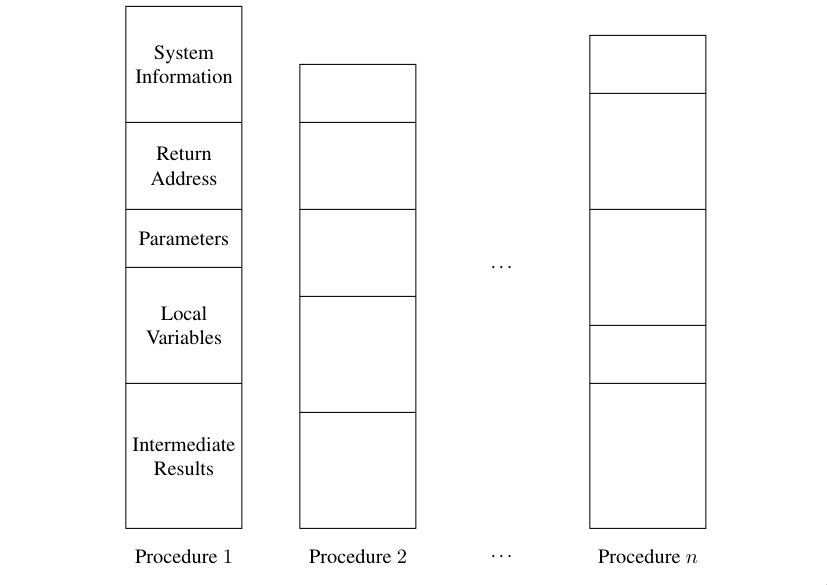
\includegraphics[width=0.5\textwidth]{img/2025-03-02-10-46-16.png}
\end{center}

Questo metodo funziona solo se siamo sicuri che, se una procedura e' attiva, allora non puo' chiamare la stessa procedura ricorsivamente. Questo e' perche' esiste solo un'istanza per ogni procedura allocata in memoria e non e' possibile sapere quante volte una funzione verra' chiamata ricorsivamente. Quindi, se vogliamo implementare la ricorsione, serve l'allocazione \textit{dinamica} (stack di chiamate):

\section{Allocazione Dinamica}
\subsection{Allocazione Dinamica con Pila}

Ogni istanza di sottoprogramma viene memorizzata con un \textit{frame} (o \textit{record di attivazione}) che contiene tutte le informazioni necessarie. Quando un'istanza viene attivata, il relativo frame viene messo in cima a una \textbf{pila}, la struttura dati naturale in quanto se una procedura A chiama una procedura B, allora siamo sicuri che B deve terminare prima che A possa continuare l'esecuzione e terminare anch'esso.

\nt{
  L'allocazione dinamica e' utile anche quando non c'e' ricorsione come meccanismo per risparmiare memoria.
}

Vediamo un esempio:

\begin{lstlisting}[language=C]
A:{
  int a = 1;
  int b = 0;

  B:{
    int c = 3;
    int b = 3;
  }
  b = a + 1;
}
\end{lstlisting}

\begin{center}
  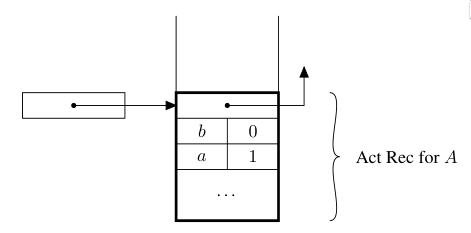
\includegraphics[width=0.3\textwidth]{img/2025-03-02-11-40-29.png}
  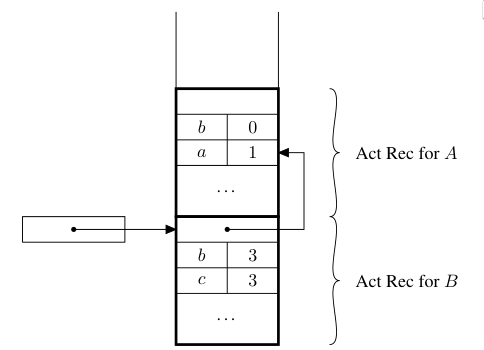
\includegraphics[width=0.3\textwidth]{img/2025-03-02-11-41-09.png}
  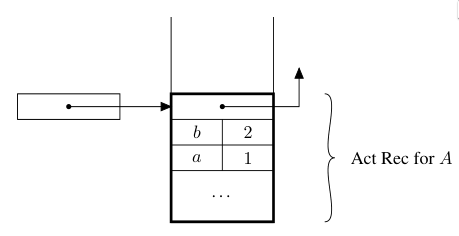
\includegraphics[width=0.3\textwidth]{img/2025-03-02-11-42-23.png}
\end{center}

Vediamo piu' in dettaglio cosa viene memorizzato nei record di attivazione:

\subsubsection{Record di attivazione}
Per un semplice blocco anonimo, il corrispondente frame ha tale forma:
\begin{center}
    \renewcommand{\arraystretch}{2} % Increase row height
    \setlength{\tabcolsep}{2em} % Adjust column spacing
    
    \begin{tabular}{|c|}
        \hline
        \textbf{Dynamic chain pointer} \\ \hline
        \textbf{Local variables} \\ \hline
        \textbf{Intermediate results} \\ \hline
    \end{tabular}
\end{center}

\nt{
  Nella realta' la maggior parte dei linguaggi usa l'allocazione statica per blocchi anonimi per maggiore efficenza di calcolo (sacrificando pero' l'efficenza di memoria).
}

Mentre per le procedure e' un po' piu' complesso:
\begin{center}
    \renewcommand{\arraystretch}{1.8} % Increase row height for better spacing
    \setlength{\tabcolsep}{2em} % Adjust column spacing
    
    \begin{tabular}{|c|}
        \hline
        \textbf{Dynamic Chain Pointer} \\ \hline
        \textbf{Static Chain Pointer} \\ \hline
        \textbf{Return Address} \\ \hline
        \textbf{Address for Result} \\ \hline
        \textbf{Parameters} \\ \hline
        \textbf{Local Variables} \\ \hline
        \textbf{Intermediate Results} \\ \hline
    \end{tabular}
\end{center}

Vediamo in dettaglio cosa sono tutti sti dati:
\begin{itemize}
\item \textbf{Intermediate Results}: serve per memorizzare risultati intermedi di equazioni complicate e per risultati di chiamate ricorsive.
\item \textbf{Local Variables} e \textbf{Parameters}: per le variabili locali e parametri.
\item \textbf{Dynamic Chain Pointer}: puntatore all'ultimo RdA creato sulla stack, l'insieme di tutti i puntatori dinamici e' chiamata \textit{catena dinamica}.
\item \textbf{Static Chain Pointer}: informazione necessaria per implementare lo scope statico, vedremo piu' avanti.
\item \textbf{Return Address}: indirizzo di memoria della prima istruzione da eseguire quando termina la procedura corrente.
\item \textbf{Address for Result}: indirizzo dove puo' essere salvato il valore di ritorno della funzione (sara' un indirizzo interno al frame della funzione chiamante).
\end{itemize}

\subsubsection{Gestione della Pila}

Vediamo la struttura di un sistema a pila (discendente):
\begin{center}
  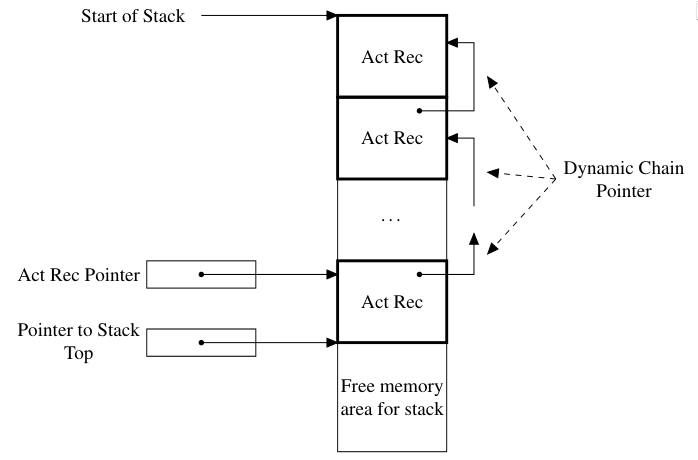
\includegraphics[width=0.5\textwidth]{img/2025-03-02-12-39-06.png}
\end{center}

Come puo' notare dall'immagine, ci sono due puntatori esterni che puntano a posti specifici sull'ultimo record di attivazione:
\begin{itemize}
  \item \textbf{Pointer al RdA}: e' un puntatore ad un luogo predeterminato all'interno del frame usato come base da cui si puo' calcolare l'offset per accedere alle variabili locali. Questo offset e' determinabile staticamente dal compilatore (ad eccezzione del caso di variaili di dimensione variabile).
\item \textbf{Stack Top Pointer}: come si puo' indovinare, e' il puntatore al primo indirizzo libero di memoria dopo l'ultimo RdA. Puo' essere omesso se e' possibile calcolare lo stesso indirizzo partendo dal pointer al RdA.
\end{itemize}

Il funzionamento corretto della pila di RdA e' dato dalla collaborazione fra il chiamante e il blocco chiamato, che eseguono dei blocchi di codice inseriti dal compilatore (o interprete) prima e dopo chiamate a procedure e blocchi anonimi:
\begin{itemize}
\item \textbf{Sequenza di Chiamata}: eseguito dal chiamante subito prima della chiamata
\item \textbf{Prologo}: eseguito immediatamente all'inizio del blocco chiamato
\item \textbf{Epilogo}: eseguito alla fine del blocco
\item \textbf{Sequenza di Ritorno}: eseguito dal chiamante immediatamente dopo la chiamata
\end{itemize}

Al momento della chiamata, la Sequenza di Chiamata e il Prologo devono:
\begin{itemize}
\item \textbf{Modificare PC}
\item \textbf{Allocare spazio sulla pila}
\item \textbf{Modifica pointer RdA}
\item \textbf{Passaggio parametri}
\item \textbf{Memorizzare registri}
\end{itemize}

Quado il blocco o processo chiamato termina, l'Epilogo e la Sequenza di Ritorno devono:
\begin{itemize}
\item \textbf{Modificare PC}
\item \textbf{Ritornare Valori}
\item \textbf{Recuperare Registri}
\item \textbf{Deallocare spazio sulla pila}
\end{itemize}

\nt{
  Sono stati omessi meccanismi per l'implementazione delle regole di scope. Vedremo queste piu' avanti.
}

\subsection{Allocazione Dinamica con Heap}

Nel caso in cui vogliamo dare la possibilita' a chi usa il linguaggio di allocare esplicitamente memoria a run-time o di usare oggetti di dimensioni variabili sorge il seguente problema: la vita degli oggetti non e' per forza LIFO, ovvero un oggetto creato prima di un altro puo' essere rimosso dalla memoria prima di un'altro oggetto creato dopo, come nel seguente blocco di codice:

\begin{lstlisting}[language=C]
  int *p, *q;
  p = malloc(sizeof(int));
  q = malloc(sizeof(int));
  *p = 0;
  *q = 1;
  free(p);
  free(q);
\end{lstlisting}

Dobbiamo usare quindi la \textit{heap}, ovvero una regione di memoria i cui blocchi possono essere allocati/deallocati in momenti arbitrari.

\nt{
  La heap che abbiamo appena definito non centra niente con la struttura dati usata per la "heap sort".
}

Esistono due categorie principali di metodi di gestione della heap a seconda della lunghezza dei blocchi che memorizza, che possono essere di \textit{dimensione fissa} o \textit{variabile}.

\subsubsection{Dimensione fissa}

La heap viene suddivisa in blocchi di dimensione fissa abbastanza limitata che sono inizialmente collegati tutti assieme nella \textit{lista libera}:
\begin{center}
  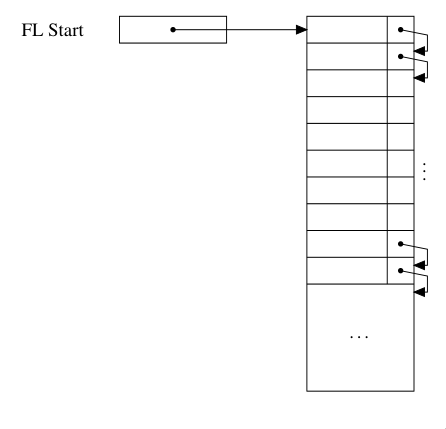
\includegraphics[width=0.3\textwidth]{img/2025-03-02-15-29-56.png}
\end{center}

A run-time, quando viene richiesto un blocco di memoria, il primo elemento della lista libera viene rimosso e restituito al processo che ha richiesto la memoria, mentre la testa della lista libera si sposta al prossimo elemento della lista. Vediamo un esempio di heap a dimensione fissa dopo alcune operazioni di allocazione/deallocazione (i blocchi grigi sono in uso):
\begin{center}
  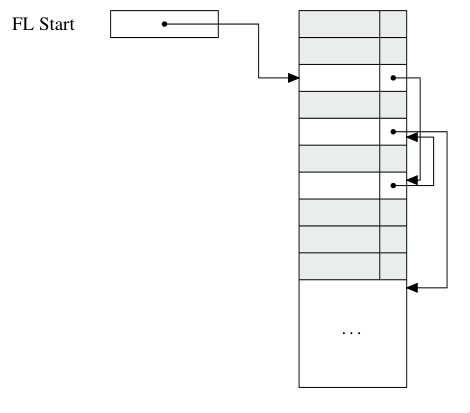
\includegraphics[width=0.3\textwidth]{img/2025-03-02-15-32-35.png}
\end{center}

\subsubsection{Dimensione variabile}

Nel caso volessimo poter allocare array la cui dimensione e' determinata solo a runtime, la soluzione a dimensione fissa non sarebbe adeguata, dato che l'array puo' essere di dimensioni maggiori rispetto ai blocchi fissi e non si possono allocare piu' blocchi perche' la memoria deve essere per forza contigua. 

In questi casi e' necessario poter richiedere un blocco di dimensione arbitraria. In un sistema di questo tipo, bisogna prestare attenzione ad usare \textit{operazioni efficenti} e a limitare lo \textit{spreco di memoria} che puo' avvenire in due situazioni:
\begin{itemize}
\item \textbf{Frammentazione interna}: viene richiesto un blocco di dimensione $ n $ ma ne viene restituito uno di dimensione $ k > n $, quindi $ k-n $ parole si perdono.
\item \textbf{Frammentazione esterna}: lo spazio totale nella memoria sarebbe abbastanza per soddisfare una richista di dimensione $ n $, ma i blocchi liberi sono separati o non contigui.
  \begin{center}
    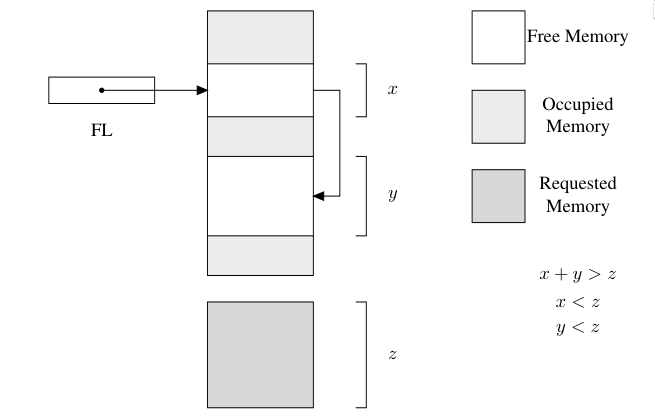
\includegraphics[width=0.4\textwidth]{img/2025-03-02-16-01-30.png}
  \end{center}
\end{itemize}

Esistono due meccanismi diversi per gestire blocchi di dimensione variabile:
\begin{itemize}
\item \textbf{Unica lista}: 

  Inizialmente, la lista libera e' composta da un solo blocco che occupa tutta la heap. Quando viene fatta la richiesta per un blocco di dimensione $ n $, le prime $ n $ parole dell'heap vengono allocate e l'inizio della lista si sposta di $ n $. Si va avanti cosi' finche' la memoria rimasta dall'inizio della lista libera alla fine della heap non e' abbastanza per soddisfare la richiesta. In queslto caso dobbiamo riutilizzare memoria deallocata, che puo' essere fatto in due modi:
    \begin{itemize}
      \item \textbf{Uso diretto della lista libera}: si scorre lungo la lista finche' si trova un blocco di dimensioni $ k > n $. Se la differenza fra la grandezza del blocco e della memoria effettivamente usata e' maggiore di una tolleranza, allora il blocco viene diviso ed il blocco di dimensione $ k - n $ viene reinserito nella lista. Possono essere usate due politiche di ricerca diverse per scegliere quale blocco prendere: \textit{first fit} e \textit{best fit}. Quando un blocco viene deallocato, si guarda se blocchi adiacenti sono anch'essi liberi e in caso affermativo si fondono per formare un blocco piu' grande (\textit{compattazione parziale}).
      \item \textbf{Compattazione della memoria libera}: tutti i blocchi attivi vengono spostati alla fine della heap, molto efficente ma funziona solo quando possiamo spostare la memoria.
    \end{itemize}
  \item \textbf{Liste libere Multiple}:

    Per ridurre il costo operativo di cercare un blocco di dimensione arbitraria, e' possibile utilizzare diverse liste per diverse dimensioni di blocchi. Quando viene richiesto un blocco di dimensione $ n $, si scorrono le liste finche' una che contiene blocchi di dimensioni adeguate non e' vuota. Anche in questo caso e' possibile riudurre la dimensione dei blocchi per ridurre la frammentazione interna, esistono due metodi:
    \begin{itemize}
      \item \textbf{Buddy system}: la dimensione dei blocchi aumenta per potenze di 2. Si calcola l'intero minore $ k $ tale che $ 2^k \geq n $ e si controlla se la relativa lista ha blocchi liberi. Altrimenti, si va a cercare nella lista $ k+1 $ e si divide il blocco in due blocchi da $ 2^k $ (la dimensione che volevamo), uno viene allocato e l'altro viene spostato nella lista corretta. Quando viene deallocato, la meta' cerca il suo compagno nella lista libera e se lo trova si uniscono e tornano nella lista originale.
      \item \textbf{Fibonacci}: funzionamento equivalente ma le dimensioni dei blocchi seguono la sequenza di Fibonacci, che sale piu' lentamente quindi porta a meno frammentazione ma piu' tempo.
    \end{itemize}
\end{itemize}

TODO: disegni esplicativi

\section{Implementazione delle Regole di Scope}

Ora che abbiamo capito come viene gestita la memoria di un programma dal compilatore, soprattuto per quanto riguarda i RdA, vediamo come possiamo implementare le regole di scope quando un blocco deve accedere a variabili non-locali.

\subsection{Scope Statico}

Se vengono implementate le regole di scope statico, allora l'ordine da seguire quando stiamo cercando il valore di una variabile non-locale non e' necessariamente quello dettato dalla catena dinamica, ovvero l'ordine delle chiamate. Infatti, l'RdA corretto e' determinato dalla struttura statica (testuale) del programma, seguendo quindi l'ordine di annidamento dei blocchi. Vediamo un esempio:

\begin{center}
  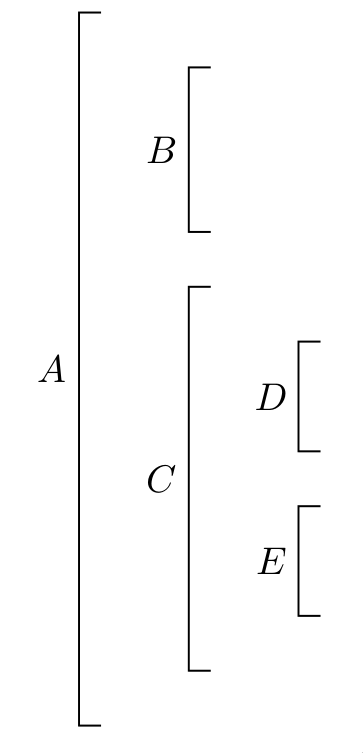
\includegraphics[width=0.1\textwidth]{img/2025-03-06-11-36-18.png}
\end{center}

Data la stuttura soprastante, immaginiamo di chiamare in ordine $ A,B,C,D,E,C $ e che rimangano tutte attive:
\begin{itemize}
\item Aggiungiamo inizialmente l'RdA di $ A $ allo stack di sistema, aggiornando lo SP e l'RdA pointer. Dato che e' il primo sulla pila, non ha nessun link.
\item Man mano che aggiungo i RdA di $ B,C,... $ aggiorno sempre SP e RdA pointer, ma e' anche necessario determinare il link dinamico e statico.
\end{itemize}

Quindi con tutte le chiamate aperte la situazione e' questa:
\begin{center}
  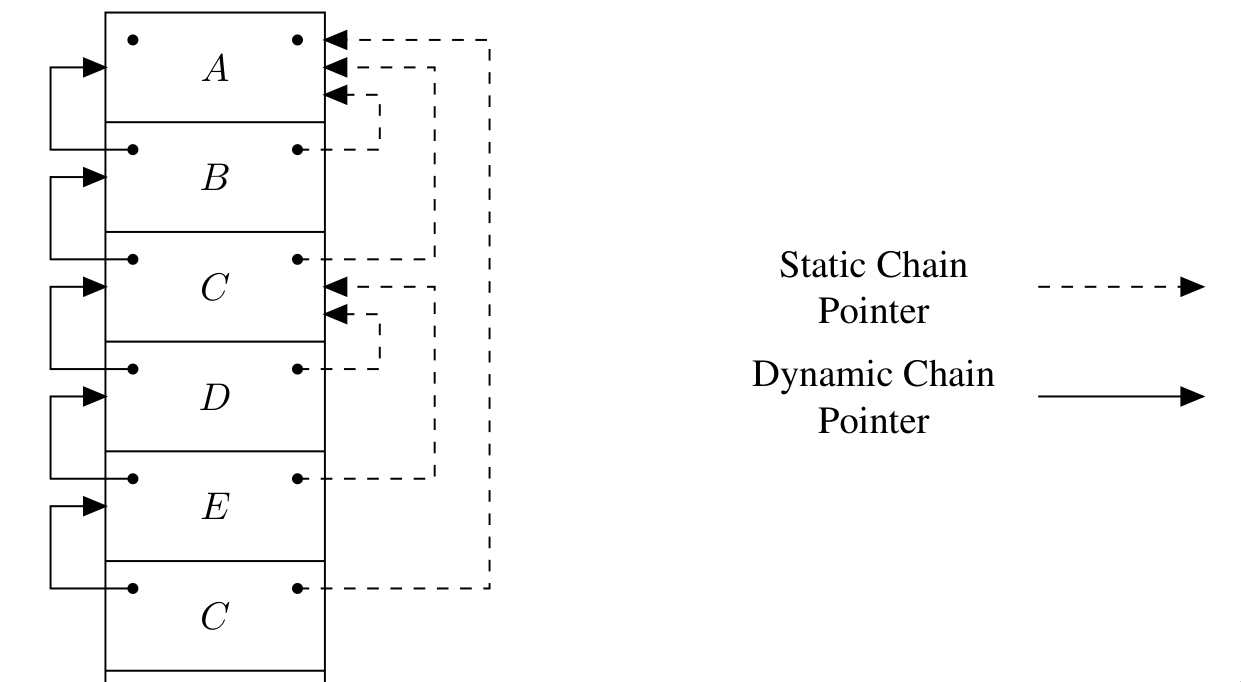
\includegraphics[width=0.5\textwidth]{img/2025-03-06-11-42-43.png}
\end{center}

Come al solito, il puntatore di catena dinamica punta all'RdA \textit{temporalmente precedente} (quello appena sotto nella pila), mentre il puntatore di catena \textbf{statica} indica l'RdA del blocco che \textit{contiene strutturalmente} quello in cui siamo.

\nt{
  Se un sottoprogramma e' annidato a livello k, allora la catena statica sara' lunga k.
}

Supponiamo di essere in $ E $ e di voler accedere alla variabile $ x $ in modo statico dichiarata in $ A $:
\begin{itemize}
\item Seguendo la catena statica, controllo se $ x $ e' dichiarata in $ C $.
\item Non c'e', quindi continuo a seguire i link statici e arrivo in $ A $, dove trovo il valore cercato.
\end{itemize}

Il supporto a run-time della catena statica e' compito della sequenza di chiamata, prologo e l'epilogo che abbiamo visto prima per le chiamate. L'approccio piu' comune e' quello dove il chiamante calcola il puntatore a catena statica che passa poi al chiamato, e' abbastanza semplice e puo' essere diviso in due casi:

\begin{itemize}
  \item \textbf{Il chiamato e' esterno al chiamante}: secondo le regole di visibilita', questa situazione e' possibile solo se il chiamante e' annidato internamente rispetto al blocco del chiamato. Cio' significa che tale blocco e' ancora attivo sulla pila, come tutti i blocchi annidati fino a quello del chiamante. Dato che sappiamo il livello di annidamento di ciascun blocco (puo' essere calcolato staticamente), basta trovare la differenza fra il livello del chiamante meno il chiamato e fare questo numero di salti sulla catena statica del chiamante (che e' in cima alla stack). In questo modo ci troviamo nel RdA del blocco contenente la definizione del chiamato, e ci basta solo passare l'indirizzo di tale RdA al chiamato che lo imposta come link statico.
    \begin{center}
      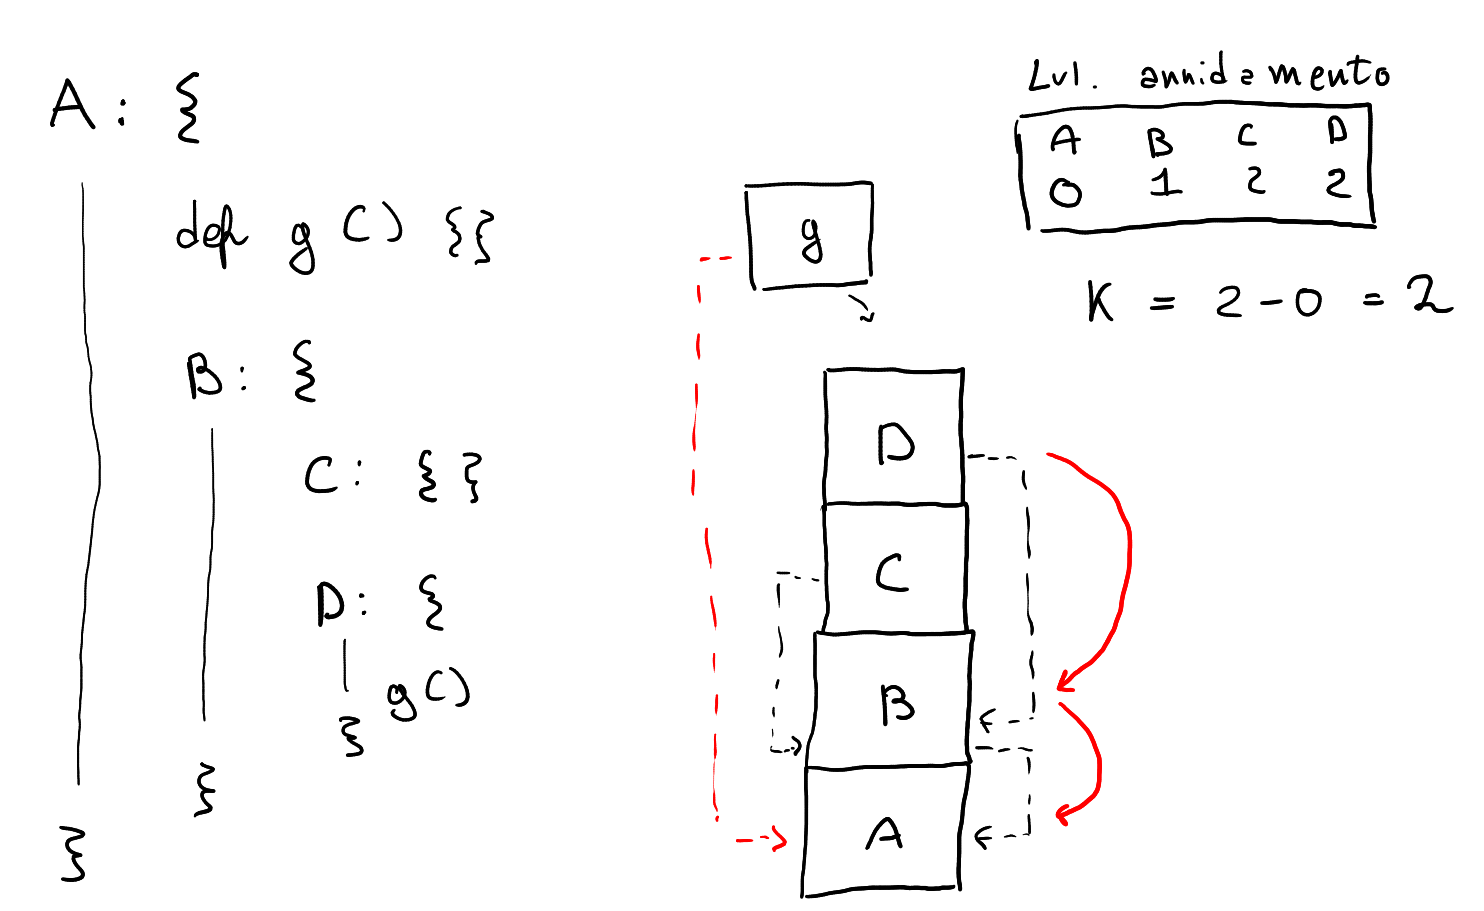
\includegraphics[width=0.3\textwidth]{img/2025-03-06-14-23-08.png}
    \end{center}
  \item \textbf{Il chiamato e' interno al chiamante}: tale situazione puo' succedere solo se il chiamato e' definito nello stesso blocco dove viene chiamato. Siamo quindi in un caso speciale del punto precedente dove la distanza di annidamento e' 0, quindi basta passare come link statico al chiamato il puntatore RdA del record contenente la chiamata (che sara' quello in cima).
    \begin{center}
      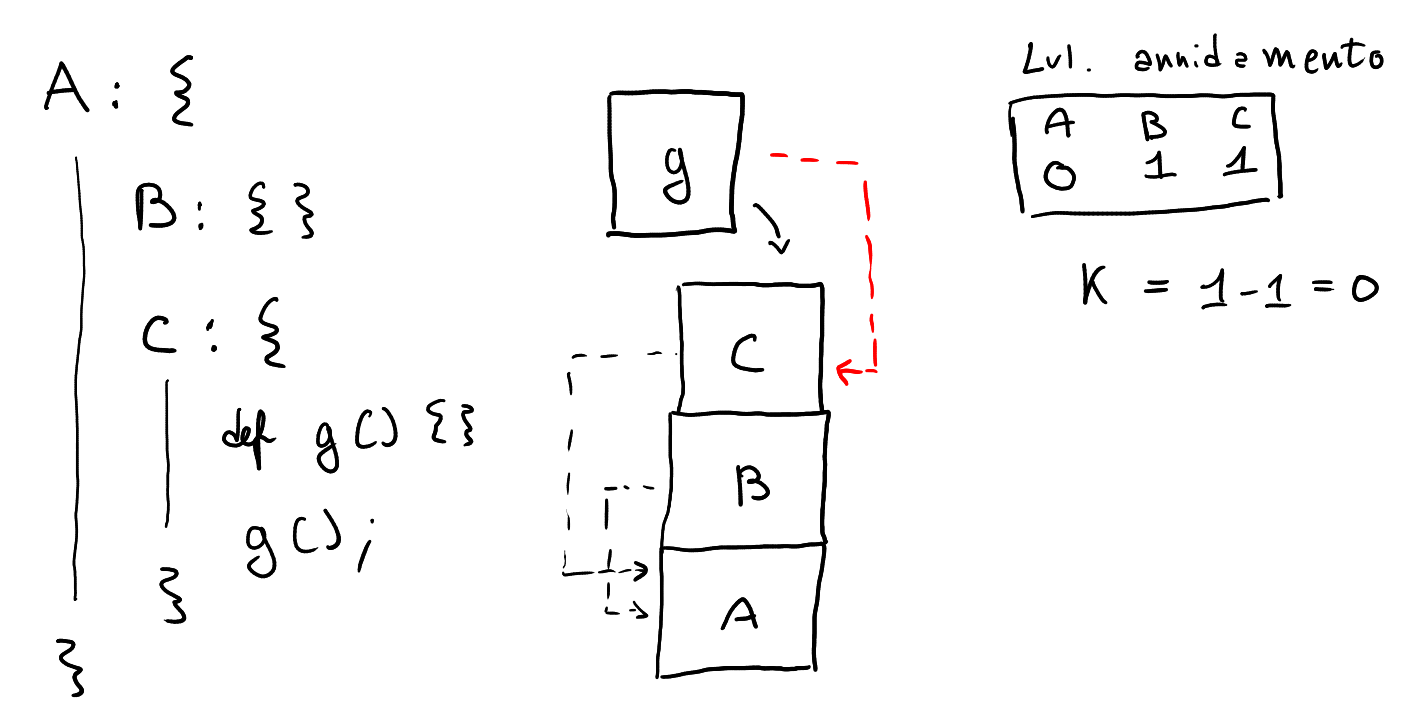
\includegraphics[width=0.3\textwidth]{img/2025-03-06-14-26-54.png}
    \end{center}
\end{itemize}

Il numero di "salti" da fare per raggiungere il RdA corretto e' calcolabile staticamente dal compiler usando la \textit{tabella dei simboli}, che memorizza anche il livello di annidamento al quale e' stata dichiarata la variabile cercata. 

Pero' non e' possibile stabilire staticamente la locazione esatta di memoria dove si trovera' tale variabile non-locale, dato che, pur sapendo il numero di "salti", non sappiamo quanti e quali RdA si trovano fra ogni salto a run-time. Per questo motivo ci serve la catena statica.

\begin{center}
  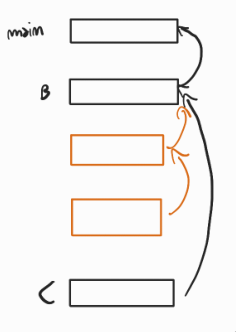
\includegraphics[width=0.2\textwidth]{img/2025-03-06-13-14-42.png}
\end{center}

\subsubsection{Il Display}

E' un po' uno schifo dover seguire sta catena statica, dato che se siamo a un livello $ k $ di annidamento, dobbiamo per forza eseguire $ k $ accessi a memoria per arrivare finalmente al frame giusto. Anche se nella pratica generalmente non e' un problema, possiamo ottimizzarlo quindi lo facciamo.

TODO: Fai Display, CRT e A-List

% \end{document}


zio pera
\end{document}
